\section{Tiến hành thí nghiệm}

Các bước thí nghiệm chung:

\begin{enumerate}
    \item Thêm nhiễu cho ảnh bằng MATLAB
    \item Xử lý nhiễu bằng MATLAB trên máy tính và xứ lý nhiễu bằng Python trên Raspberry Pi 3
    \item Lấy kết quả MATLAB làm chuẩn để đánh giá kết quả giảm nhiễu ảnh trên Raspberry Pi.
\end{enumerate}

\begin{figure}[H]
    \centering
    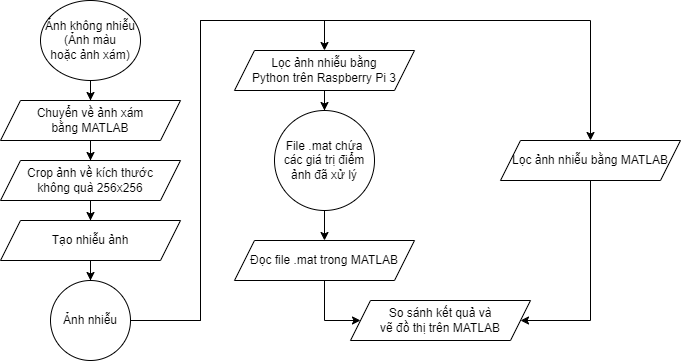
\includegraphics[width=.8\linewidth]{images/denoise_flowchart.png}
    \caption{Quy trình thí nghiệm}
    \label{fig:denoise_flowchart}
\end{figure}

\subsection{Triệt nhiễu ảnh muối tiêu}

\subsubsection{Tạo ảnh nhiễu muối tiêu trên MATLAB}

Ta đọc một ảnh gốc (ảnh màu hoặc ảnh xám), chuyển sang ảnh xám nếu cần, crop ảnh xuống $256 \times 256$ để thuận tiện cho việc xử lý. Cuối cùng, ta tạo nhiễu muối tiêu cho ảnh bằng hàm \texttt{imnoise} có sẵn của MATLAB.

\begin{figure}[H]
    \centering
    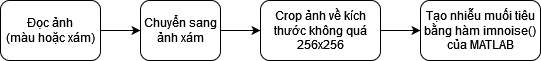
\includegraphics[width=1\linewidth]{images/salt_pepper_gen_noise.png}
    \caption{Các bước tạo ảnh nhiễu muối tiêu trên MATLAB}
    \label{fig:salt_pepper_gen_noise}
\end{figure}

\begin{lstlisting}[language=MATLAB]
figure, tiledlayout(1,2)

% Doc anh, chuyen sang anh xam, va crop anh neu kich thuoc lon hon 255
I = imread('dataset\4.1.03.tiff');
I = rgb2gray(I);
[rows, cols] = size(I);
size = [rows, cols];
if (rows > 256), I = imresize(I, [256 NaN]), end;
if (cols > 256), I = imresize(I, [NaN 256]), end;

% Luu anh xam da crop va hien thi anh
imwrite(I, 'images/salt_pepper_orig.bmp')
nexttile, imshow(I), title('Anh goc')

% Them nhieu muoi tieu voi mat do 0.05
J = imnoise(I, 'salt & pepper', 0.05);

% Luu anh da duoc tao nhieu va hien thi anh
imwrite(J, 'images/salt_pepper_noise.bmp')
nexttile, imshow(J), title('Anh nhieu muoi tieu 5%')
\end{lstlisting}

\begin{figure}[H]
    \centering
    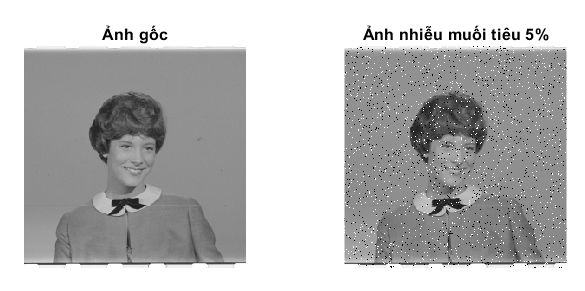
\includegraphics[width=1\linewidth]{images/salt_pepper_noise_matlab.png}
    \caption{Tạo ảnh nhiễu muối tiêu trên MATLAB}
    \label{fig:salt_pepper_noise_matlab}
\end{figure}

\subsubsection{Lọc ảnh nhiễu muối tiêu trên MATLAB}

Ta lọc ảnh bằng bộ lọc trung vị kích thước $3 \times 3$ với hàm \texttt{medfilt2()} có sẵn của MATLAB. 

Để đánh giá hiệu quả của bộ lọc, ta tính sai số bình phương trung bình (mean square error, MSE) giữa ảnh gốc và ảnh đã lọc:

\begin{equation}\label{eqn:MSE}
    MSE = \frac{1}{WH} \sum_{i=1}^{H} \sum_{j=1}^{W} {(y_{ij} - x_{ij})^2}
\end{equation}

Trong đó, $W$ và $H$ là chiều rộng và chiều cao ảnh, $x$ là ảnh gốc và $y$ là ảnh đã lọc.

\begin{lstlisting}[language=MATLAB]
figure
tiledlayout(1,3)

% Doc anh xam goc va hien thi
I = imread('images/salt_pepper_orig.bmp');
nexttile, imshow(I), title('Anh goc')

% Doc anh nhieu muoi tieu va hien thi
J = imread('images/salt_pepper_noise.bmp');
nexttile, imshow(J), title('Anh nhieu muoi tieu')

% Loc trung vi voi bo loc 3x3 bang ham medfilt2 co san va luu ket qua
K = medfilt2(J, [3 3]);
nexttile, imshow(K), title('Loc trung vi 3x3 (MATLAB)')
imwrite(K, 'images/salt_pepper_denoised_matlab.bmp')

% Sai so binh phuong trung binh giua anh goc va anh da loc
fprintf("Sai so binh phuong trung binh: %.4f\n", MSE(I, K));

% Sai so binh phuong trung binh
function out = MSE(im1, im2)
    [nRows, nCols] = size(im1);
    error = im1 - im2;
    out = sum(error.^2, 'all') / (nRows * nCols);
end
\end{lstlisting}

Kết quả chạy:

\begin{verbatim}
Sai số bình phương trung bình: 3.9574
\end{verbatim}

\begin{figure}[H]
    \centering
    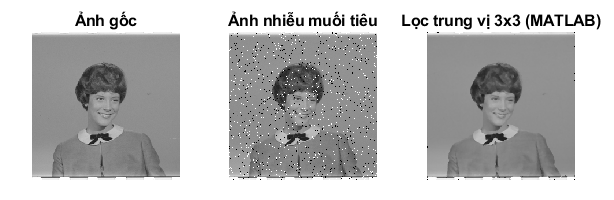
\includegraphics[width=1\linewidth]{images/salt_pepper_denoise_matlab.png}
    \caption{Lọc ảnh nhiễu muối tiêu trên MATLAB}
    \label{fig:salt_pepper_denoise_matlab}
\end{figure}

\textbf{Nhận xét:} Kết quả lọc trung vị trên MATLAB là rất hiệu quả, ảnh đã lọc cho sai số không đáng kể so với ảnh gốc. Do đó, ta có thể dùng kết quả này để làm căn cứ đánh giá mức độ hiệu quả khi triển khai lọc nhiễu muối tiêu trên Raspberry Pi 3.

\subsubsection{Lọc ảnh nhiễu muối tiêu bằng Python trên Raspberry Pi 3}

Các bước triển khai hàm lọc trung vị kích thước $3 \times 3$ trên Python như sau (Hình \ref{fig:median_filtering_algorithm}):

\begin{itemize}
    \item Padding cho ngõ vào: Để không bỏ sót các điểm ảnh ở rìa, ta cần padding cho ảnh ngõ vào. Vì bộ lọc có kích thước 3x3, ta cần padding 1 hàng zero cho rìa trên và dưới, và padding 1 cột zero cho rìa trái và phải.

    \item Tìm trung vị: Cho vòng lặp chạy qua từng điểm ảnh. Ở mỗi vòng lặp, xếp các điểm ảnh lân cận vào một mảng, sắp xếp mảng theo thứ tự tăng dần (hoặc giảm dần), và điểm ảnh ngõ ra sẽ là phần tử ở giữa của mảng đã sắp xếp.
\end{itemize}

\begin{figure}[h]
    \centering
    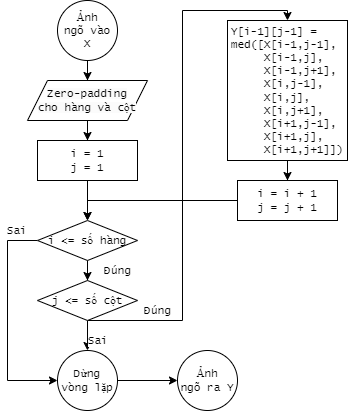
\includegraphics[width=1\linewidth]{images/median_filtering_algorithm.png}
    \caption{Thuật toán lọc trung vị}
    \label{fig:median_filtering_algorithm}
\end{figure}

Việc tìm MSE được triển khai như phương trình \ref{eqn:MSE} nêu trên.

\begin{lstlisting}[language=Python]
import cv2
import numpy as np
import matplotlib.pyplot as plt

fig, axs = plt.subplots(1, 3)

# Doc anh xam goc va hien thi
I = cv2.imread('images/salt_pepper_orig.bmp', cv2.IMREAD_GRAYSCALE)
axs[0].imshow(I, cmap='gray', vmin=0, vmax=255)
axs[0].set_title('Anh goc')

# Doc anh nhieu muoi tieu va hien thi
J = cv2.imread('images/salt_pepper_noise.bmp', cv2.IMREAD_GRAYSCALE)
axs[1].imshow(J, cmap='gray', vmin=0, vmax=255)
axs[1].set_title('Nhieu muoi tieu')

# Ham loc trung vi kich thuoc 3x3
def medFilter3x3(X):
  nRows, nCols = X.shape

  # Padding cho anh ngo vao
  hpad = np.zeros((1, nCols))
  X = np.vstack((hpad, X, hpad))
  vpad = np.zeros((nRows+2, 1))
  X = np.hstack((vpad, X, vpad))

  # Lay trung vi bang cach sap xep mang theo thu tu tang dan
  # va chon phan tu thu 5 trong 9 phan tu
  Y = np.zeros((nRows,nCols))
  for i in range(1,nRows+1):
    for j in range(1,nCols+1):
      x = [X[i-1,j-1],
           X[i-1,j],
           X[i-1,j+1],
           X[i,j-1],
           X[i,j],
           X[i,j+1],
           X[i+1,j-1],
           X[i+1,j],
           X[i+1,j+1]]
      x = sorted(x)
      Y[i-1][j-1] = x[4]
  return Y

# Sai so binh phuong trung binh
def MSE(im1, im2):
  nRows, nCols = im1.shape
  squareError = 0;
  for i in range(nRows):
    for j in range(nCols):
      squareError += (im1[i,j] - im2[i,j])**2
  return squareError / (nRows * nCols)

# Loc trung vi voi bo loc 3x3 va luu ket qua
K = medFilter3x3(J)
axs[2].imshow(K, cmap='gray', vmin=0, vmax=255)
axs[2].set_title('Loc trung vi 3x3 (RPi 3)')

# Sai so binh phuong trung binh giua anh goc va anh da loc
print("Sai so binh phuong trung binh: %.4f\n" % MSE(I,K))

# Ve cac anh
for ax in axs:
  ax.set_xticks([])
  ax.set_yticks([])

fig.tight_layout(h_pad=2)
fig.show()

# Luu anh da loc
cv2.imwrite('images/salt_pepper_denoised_rpi3.bmp', K)
\end{lstlisting}

Kết quả chạy chương trình trên Raspberry Pi 3

\begin{verbatim}
Sai số bình phương trung bình: 32.8830
\end{verbatim}

\begin{figure}[H]
    \centering
    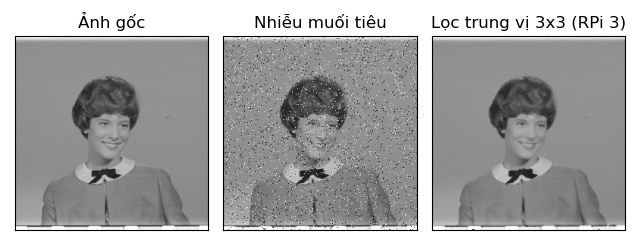
\includegraphics[width=1\linewidth]{images/salt_pepper_denoise_rpi3.png}
    \caption{Lọc ảnh nhiễu muỗi tiêu bằng Python trên Raspberry Pi 3}
    \label{fig:salt_pepper_denoise_rpi3}
\end{figure}

\textbf{Nhận xét:} Kết quả lọc trung vị bằng Python trên Raspberry Pi 3 tuy cho sai số nhiều hơn so với MATLAB, nhưng sai số này vẫn là rất nhỏ. Bằng quan sát, ảnh đã lọc trên Raspberry Pi 3 rất giống ảnh đã lọc trên MATLAB và ảnh gốc. 

\subsection{Triệt nhiễu Gauss}

\subsubsection{Tạo ảnh nhiễu Gauss}

Ta đọc một ảnh gốc (ảnh màu hoặc ảnh xám), chuyển sang ảnh xám nếu cần, crop ảnh xuống $256 \times 256$ để thuận tiện cho việc xử lý. Cuối cùng, ta tạo nhiễu muối tiêu cho ảnh bằng hàm \texttt{imnoise} có sẵn của MATLAB.

\begin{figure}[H]
    \centering
    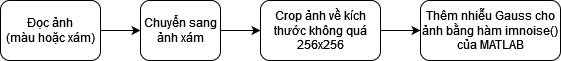
\includegraphics[width=1\linewidth]{images/gaussian_gen_noise.png}
    \caption{Các bước thêm nhiễu Gauss cho ảnh trên MATLAB}
    \label{fig:gaussian_gen_noise}
\end{figure}

\begin{lstlisting}[language=MATLAB]
figure
tiledlayout(1,2)

% Doc anh, chuyen sang anh xam, va crop anh neu kich thuoc lon hon 255
I = imread('dataset\4.2.01.tiff');
I = rgb2gray(I);
[rows, cols] = size(I);
size = [rows, cols];
if (rows > 256), I = imresize(I, [256 NaN]); end;
if (cols > 256), I = imresize(I, [NaN 256]); end;

% Luu anh xam da crop va hien thi anh
imwrite(I, 'images/gaussian_orig.bmp');
nexttile, imshow(I), title('Anh goc');

% Them nhieu Gauss voi trung binh 0, phuong sai 0.05
J = imnoise(I, 'gaussian');

% Luu anh da duoc tao nhieu va hien thi anh
imwrite(J, 'images/gaussian_noise.bmp');
nexttile, imshow(J), title('Anh nhieu Gauss mu=0, var=0.05');
\end{lstlisting}

\begin{figure}[H]
    \centering
    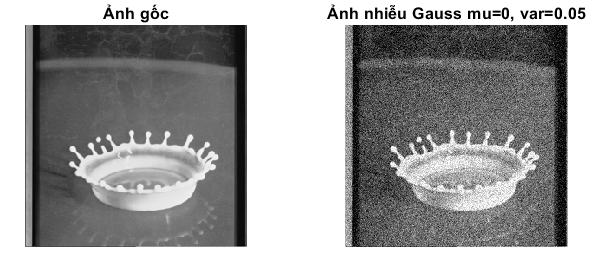
\includegraphics[width=.9\linewidth]{images/gaussian_noise_matlab.png}
    \caption{Ảnh nhiễu Gauss tạo từ MATLAB}
    \label{fig:gaussian_noise_matlab}
\end{figure}

Nếu không cung cấp thêm tham số, mặc định MATLAB sẽ tạo nhiễu Gauss trắng với trung bình $\mu = 0$ và phương sai hay công suất nhiễu $\sigma^2 = 0.01$.

\subsubsection{Lọc ảnh nhiễu Gauss trên MATLAB}

Ta lọc ảnh bằng bộ lọc Wiener với hàm \texttt{wiener2()} có sẵn của MATLAB. Wiener là bộ lọc thông thấp một hình ảnh có giá trị cường độ bị suy hao bởi nhiễu cộng có công suất hằng. Với mỗi điểm ảnh, bộ lọc sẽ tìm trung bình và độ lệch chuẩn cục bộ trong một lân cận có kích thước được định sẵn.
Nếu không cung cấp thêm tham số kích thước bộ lọc và công suất nhiễu, mặc định MATLAB sẽ dùng cửa sổ lọc có kích thước $3 \times 3$, và ước lượng công suất nhiễu trước khi thực hiện quá trình lọc.

\begin{lstlisting}[language=MATLAB]
figure
tiledlayout(1,3)

% Doc anh xam goc va hien thi
I = imread('images/gaussian_orig.bmp');
nexttile, imshow(I), title('Anh goc')

% Doc anh nhieu Gauss va hien thi
J = imread('images/gaussian_noise.bmp');
nexttile, imshow(J), title('Anh nhieu Gauss')

% Loc nhieu Gauss bang ham wiener2 co san va luu ket qua
[K, noise] = wiener2(J);
nexttile, imshow(K), title('Loc nhieu Gauss (MATLAB)')
imwrite(K, 'images/gaussian_denoised_matlab.bmp')

% Cong suat nhieu uoc luong
fprintf("Cong suat nhieu uoc luong: %.4f\n", noise);
\end{lstlisting}

\begin{verbatim}
Công suất nhiễu ước lượng: 0.0105
\end{verbatim}

\begin{figure}[H]
    \centering
    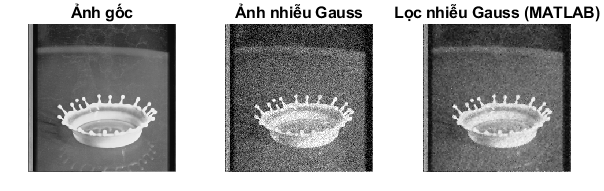
\includegraphics[width=1\linewidth]{images/gaussian_denoise_matlab.png}
    \caption{Lọc ảnh nhiễu Gauss trên MATLAB}
    \label{fig:gaussian_denoise_matlab}
\end{figure}

\textbf{Nhận xét}: Hàm \texttt{wiener2} của MATLAB ước lượng tốt công suất nhiễu (0.0105 so với 0.010), do đó cho kết quả lọc tương đối tốt. 

\subsubsection{Lọc ảnh nhiễu Gauss tiêu bằng Python trên Raspberry Pi 3}

Tương tự, với Python trên Raspberry Pi 3, ta lọc ảnh bằng bộ lọc Wiener với hàm \texttt{wiener()} của thư viện \texttt{scipy.signal}. Wiener là bộ lọc thông thấp một hình ảnh có giá trị cường độ bị suy hao bởi nhiễu cộng có công suất hằng. Với mỗi điểm ảnh, bộ lọc sẽ tìm trung bình và độ lệch chuẩn cục bộ trong một lân cận có kích thước được định sẵn.

Ta cung cấp tham số kích thước bộ lọc là $3 \times 3$ (giống kích thước trong MATLAB), nhưng không cung cấp giá trị công suất nhiễu để phần mềm tự ước lượng giá trị này. 

\begin{lstlisting}[language=Python]
import cv2
import numpy as np
import matplotlib.pyplot as plt
from scipy.signal import wiener

fig, axs = plt.subplots(1, 3)

# Doc anh xam va hien thi
I = cv2.imread('images/gaussian_orig.bmp', cv2.IMREAD_GRAYSCALE)
axs[0].imshow(I, cmap='gray', vmin=0, vmax=255)
axs[0].set_title('Anh goc')

# Doc anh nhieu Gauss va hien thi
J = cv2.imread('images/gaussian_noise.bmp', cv2.IMREAD_GRAYSCALE)
axs[1].imshow(J, cmap='gray', vmin=0, vmax=255)
axs[1].set_title('Nhieu Gauss')

# Loc nhieu Gauss bang ham scipy.signal.wiener co san (tham so mac dinh) va luu ket qua
K = wiener(J, (3,3))
axs[2].imshow(K, cmap='gray', vmin=0, vmax=255)
axs[2].set_title('Loc nhieu Gauss \n (RPi 3, mac dinh)')

# Ve cac anh
for ax in axs:
  ax.set_xticks([])
  ax.set_yticks([])

fig.tight_layout(h_pad=2)
fig.show()

# Luu anh da loc
cv2.imwrite('images/gaussian_denoised_rpi3.bmp', K)
\end{lstlisting}

\begin{figure}[H]
    \centering
    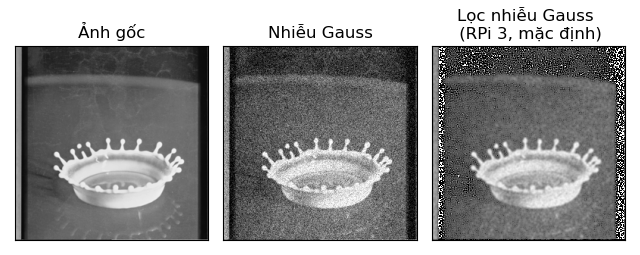
\includegraphics[width=1\linewidth]{images/gaussian_denoise_rpi3_default.png}
    \caption{Lọc ảnh nhiễu Gauss bằng hàm scipy.signal.wiener() trên Python trên Raspberry Pi 3 (tham số mặc định)}
    \label{fig:gaussian_denoise_rpi3_default}
\end{figure}

\textbf{Nhận xét}: Kết quả lọc nhiễu tương đối kém so với MATLAB.

Ta thử lại, cung cấp thêm tham số công suất nhiễu đã biết trước cho hàm \texttt{wiener()} bằng cách thay thế dòng lệnh sau:

\begin{lstlisting}[language=Python]
# K = wiener(J, (3,3))
K = wiener(J, (3,3), 0.01)
\end{lstlisting}

\begin{figure}[H]
    \centering
    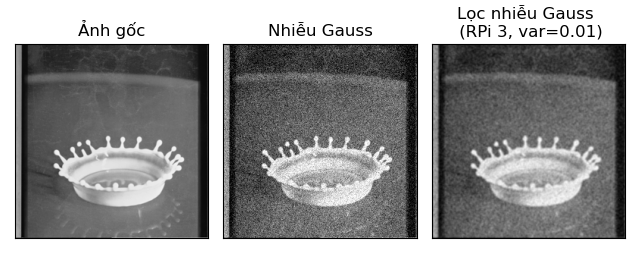
\includegraphics[width=1\linewidth]{images/gaussian_denoise_rpi3_var0p01.png}
    \caption{Lọc ảnh nhiễu Gauss bằng hàm scipy.signal.wiener() trên Python trên Raspberry Pi 3 (cung cấp tham số công suất nhiễu)}
    \label{fig:enter-label}
\end{figure}

\textbf{Nhận xét}: Khả năng ước lượng công suất nhiễu của thư viện scipy kém, dẫn đến kết quả lọc chưa tốt nếu không cung cấp tham số này. Với tham số công suất nhiễu được cung cấp, bộ lọc tỏ ra hiệu quả và kết quả lọc rất gần với kết quả của MATLAB và ảnh gốc.